\section{Implementation}

\begin{wrapfigure}{l}{0.5\textwidth}
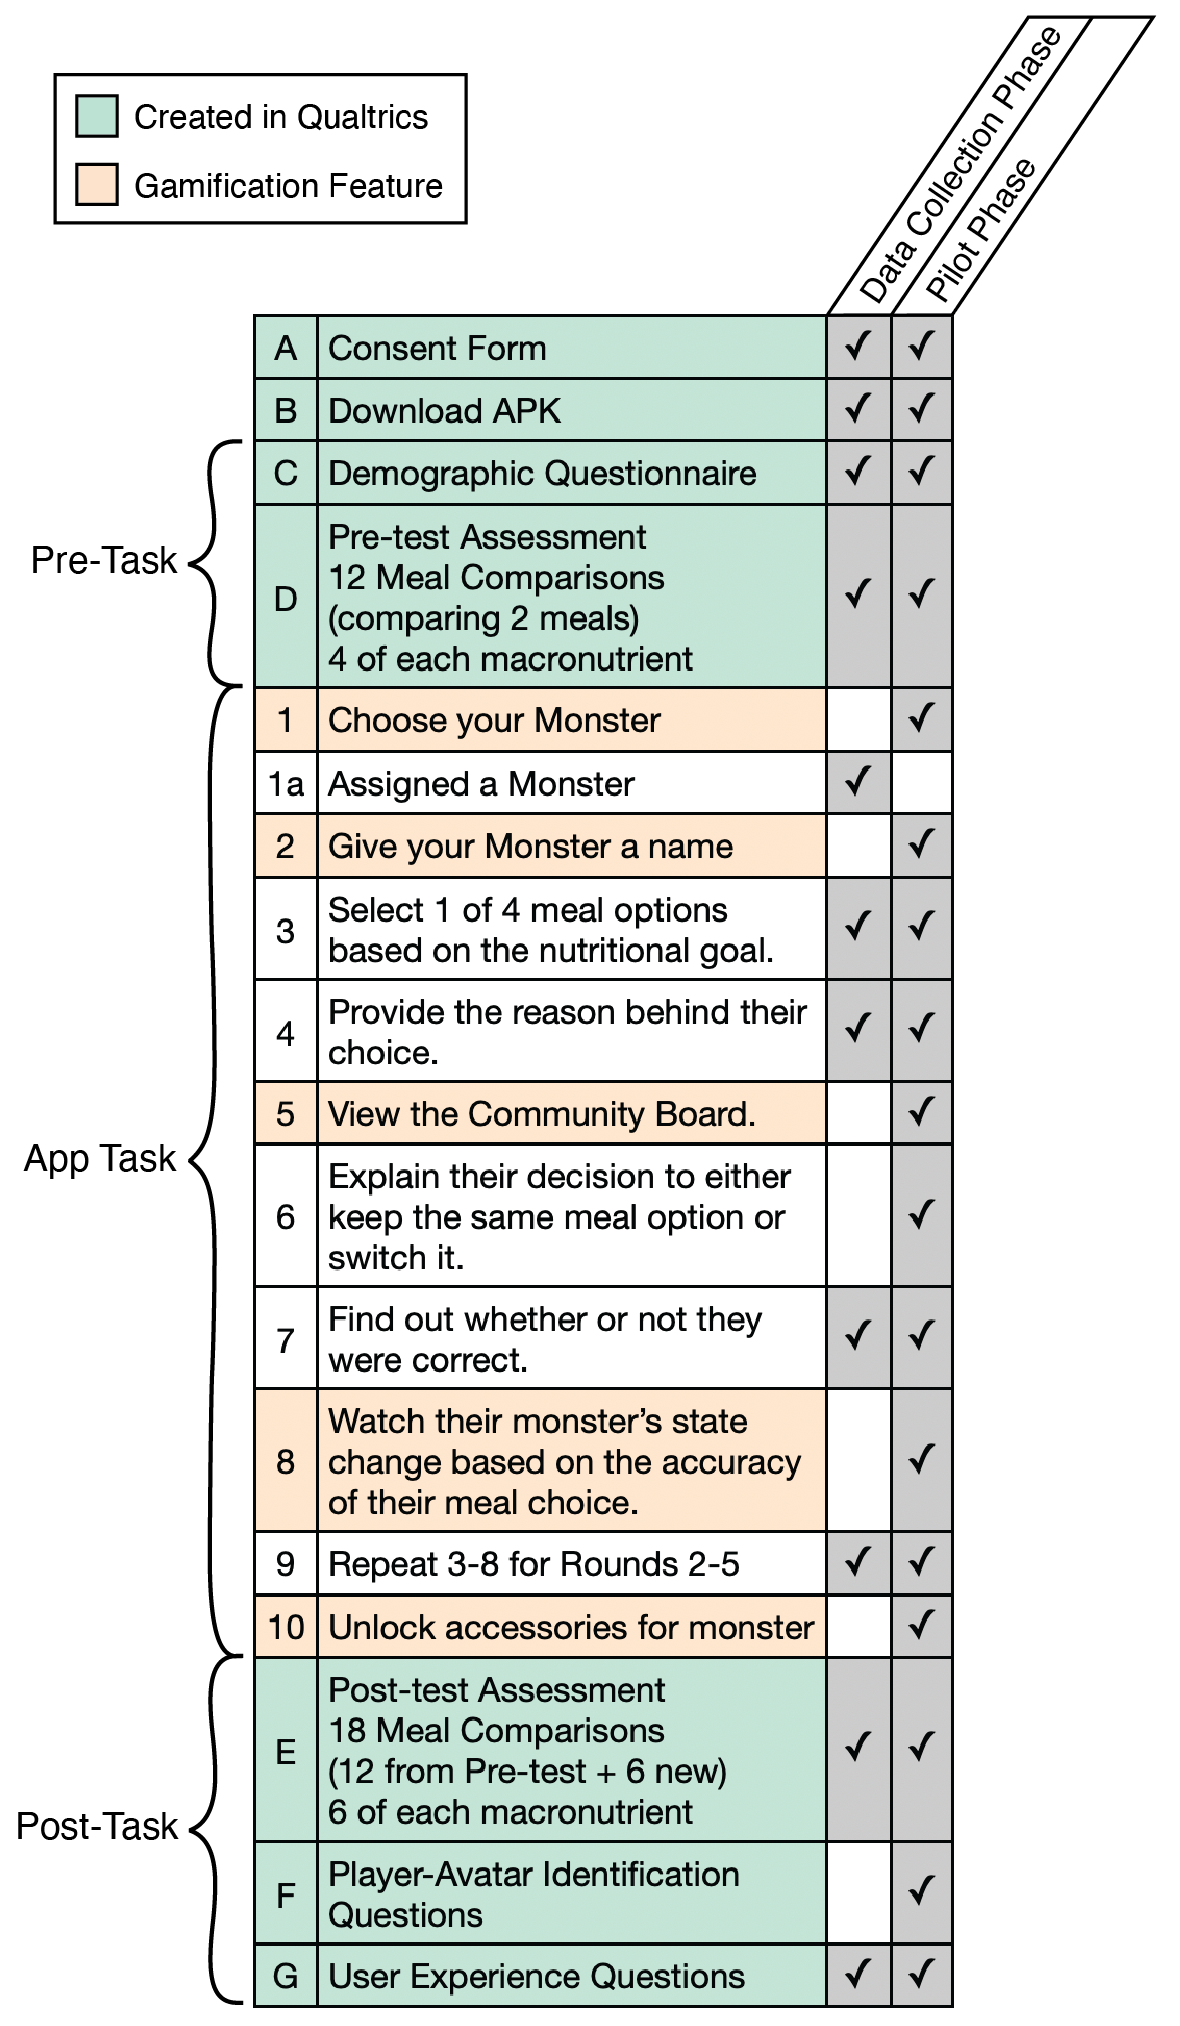
\includegraphics[width=\linewidth]{samples/images/figure-2-02.png}
\caption{Chart showing the steps of the study and the differences between the data collection phase and the experimental phase.}
\label{fig:phasechart}
\end{wrapfigure}

In this section, we outline the processes of preparing the tools we used in our study, including the survey elements of the pre-app task and post-app task, as well as the app itself.

\subsection{Development of the App}

The app was created using the visual programming interface, MIT App Inventor 2, version nb185a, and exported as a Android Package Kit using MIT App Inventor Code, version code36. An Android Package Kit (APK) is a file format used by Android to distribute and install apps.
%%Due to the 10MB APK limit in AI2, after we created the app, we had to export it as an .aia file, the native format for App Inventor apps. To build the APK, the .aia file was then imported into MIT App Inventor Code, version code36, which has a capacity for building APK files up to 50MB. 

The app was programmed to collect detailed logs of users' interactions (i.e., clicks, time-stamps) to assist in identifying user behavior and level of interaction. 
The app also randomized the meal choices within each round, as well as the order of the rounds themselves.



\subsection{Meal Photo Selection}
The app features 37 photographs of ``in-the-wild'' meals.
\textcolor{blue}{The images were gathered from a set used in one of the researchers prior crowdsourcing-in-nutrition~\cite{desai2019personal,mitchell2019wish} studies for which the expert nutritional assessment provided by a professional dietitian was available. HOW DO WE PHRASE THIS??}
We filtered the images based on their resolution quality and content clarity, so that users were able to easily identify the components of the meals.

In each round, users were presented with four ``in-the-wild'' meal photographs.
We created the rounds so that each round consisted of one best choice, one second best choice, and two less desirable choices, ranked as such by their macronutrient content assessment. 

%%-- filtering the ``in-the-wild'' meal photographs
%%-- nutrition experts helping us choose meals and or reasons (creating a ground truth)
  
%(MENTION THAT THE IMAGES ARE FROM MEALYZER AND THEN REFERENCE GLUCOGOAILIE OR GLUCORACLE STUDY -- so that we can say they are from our previous studies)


We tested the accuracy of the meal choice rankings by circulating all rounds to nutrition experts. 
We then adjusted the rounds as necessary to achieve above 50\% expert agreement for all rounds. 



\begin{figure}[h]
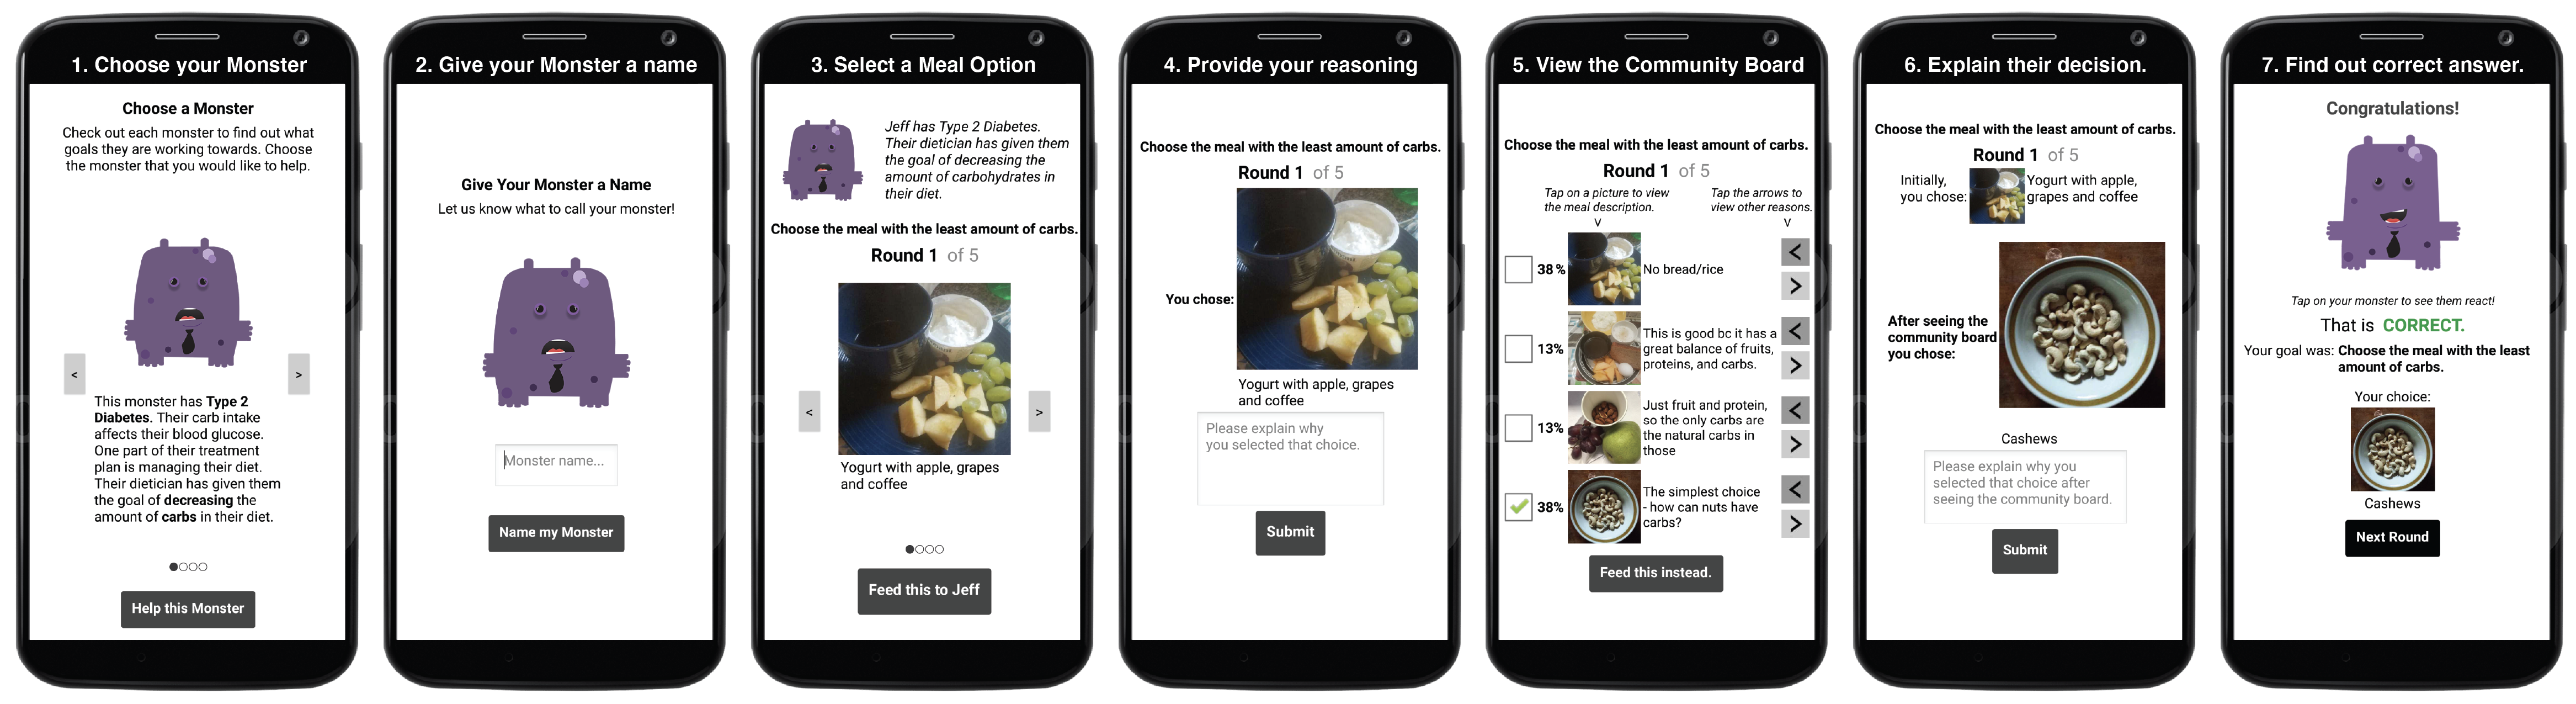
\includegraphics[width=\textwidth]{samples/images/figure-3.png}
\caption{Series of screenshots showing the main steps of the app.}
\label{fig:screenshots}
\end{figure}

%-- to refer to some figures as you explain the steps of the game
%-- game design choices
%-- why four meals per round than more
%-- connection to firebase


%The four stories were: 1) This monster has Type 2 Diabetes. Their carb intake affects their blood glucose. One part of their treatment plan is managing their diet. Their dietitian has given them the goal of decreasing the amount of carbs in their diet. 2) This monster is clinically overweight. They want to lose weight and become more healthy. One part of their plan is managing their diet.  Their dietitian has given them the goal of decreasing the fat content in their diet. 3) This monster has been training to run a marathon. Their big race is coming up. One part of their plan is managing their diet. Their dietitian has given them the goal of increasing the amount of carbs in their diet. and 4) This monster has Irritable Bowel Syndrome. Their daily life is greatly influenced by the way their digestive system behaves. One part of their treatment plan is managing their diet. Their dietitian has given them the goal of increasing the amount of fiber in their diet. 


\subsection{Gamification Features}
The Experimental Phase (EP) differed from the Data Collection Phase (DCP) with inclusion of Gamification Features (GF). 
%The GF occur throughout the game-play of the app. 
They can be seen within the context of the app and larger study flow in Figure~\ref{fig:phasechart}.

\subsubsection{GF1: The Ability for the User to Select and Name a Pet Monster Avatar}

There are four monsters in the app, each having their own brief background story as to why they are pursuing their nutritional goal. 
For example, one monster's story reads: \textit{This monster has Irritable Bowel Syndrome. Their daily life is greatly influenced by the way their digestive system behaves. One part of their treatment plan is managing their diet. Their dietitian has given them the goal of increasing the amount of fiber in their diet}. 

In the DCP, users were assigned to their monster and provided with its story and corresponding nutritional goal. 
In the EP, users could choose their own monster avatar with a corresponding health goal. After selecting one of the four monsters, users were asked to give their monster a name. 
This custom name was used throughout the rest of the game. 
Figure~\ref{fig:screenshots} shows screenshots of the app with the steps of the ``gameplay.'' 
Screen 1 is where users can tap through the carousel of monster choices to choose a monster to play with. Screen 2 shows how a user can give their monster avatar a custom name. The subsequent screens show an example of playing Round 1, where the custom name (e.g., ``Jeff'') can be seen implemented in the game.

\subsubsection{GF2: Viewing the Community Board of Crowdsourced Intelligence}

The inclusion of a community board (CB) allows users to view input from other users' to assist them in deciding which meal best fits the chosen nutritional goal. 
This CB displays both the percentage of users that selected each of the four meal options as well as three user-generated reasons as to why other users chose that meal option. The presented user-generated reasons were from those collected in the DCP. 
\textcolor{blue}{How should we explain that we also gathered "fake" reasons (with the google forms) so that every meal choice had three reasons (even if it showed 0\%)?}


%The inclusion of the community board will allow us to analyze how users decisions might be influenced by the (un)popular opinion and reasonings of other users. 
%We anticipate that in scenarios where the user is swayed by the community board and then shown to be incorrect, we will see a reluctancy in future rounds to trust the opinions of others over their own instincts. 
%However, this will most likely change when the community board helps the user find the correct answer, in which case we anticipate that it will be common to see the user trusting the opinions of others in the future.
  
\subsubsection{GF3: Monster State Change and Accessory Unlocking in Reaction to Meal Choice Accuracy}
%These gamification features provide a lightweight environment for users to gain exposure and knowledge about nutrition components of different meals.

\begin{wrapfigure}{l}{0.5\textwidth}
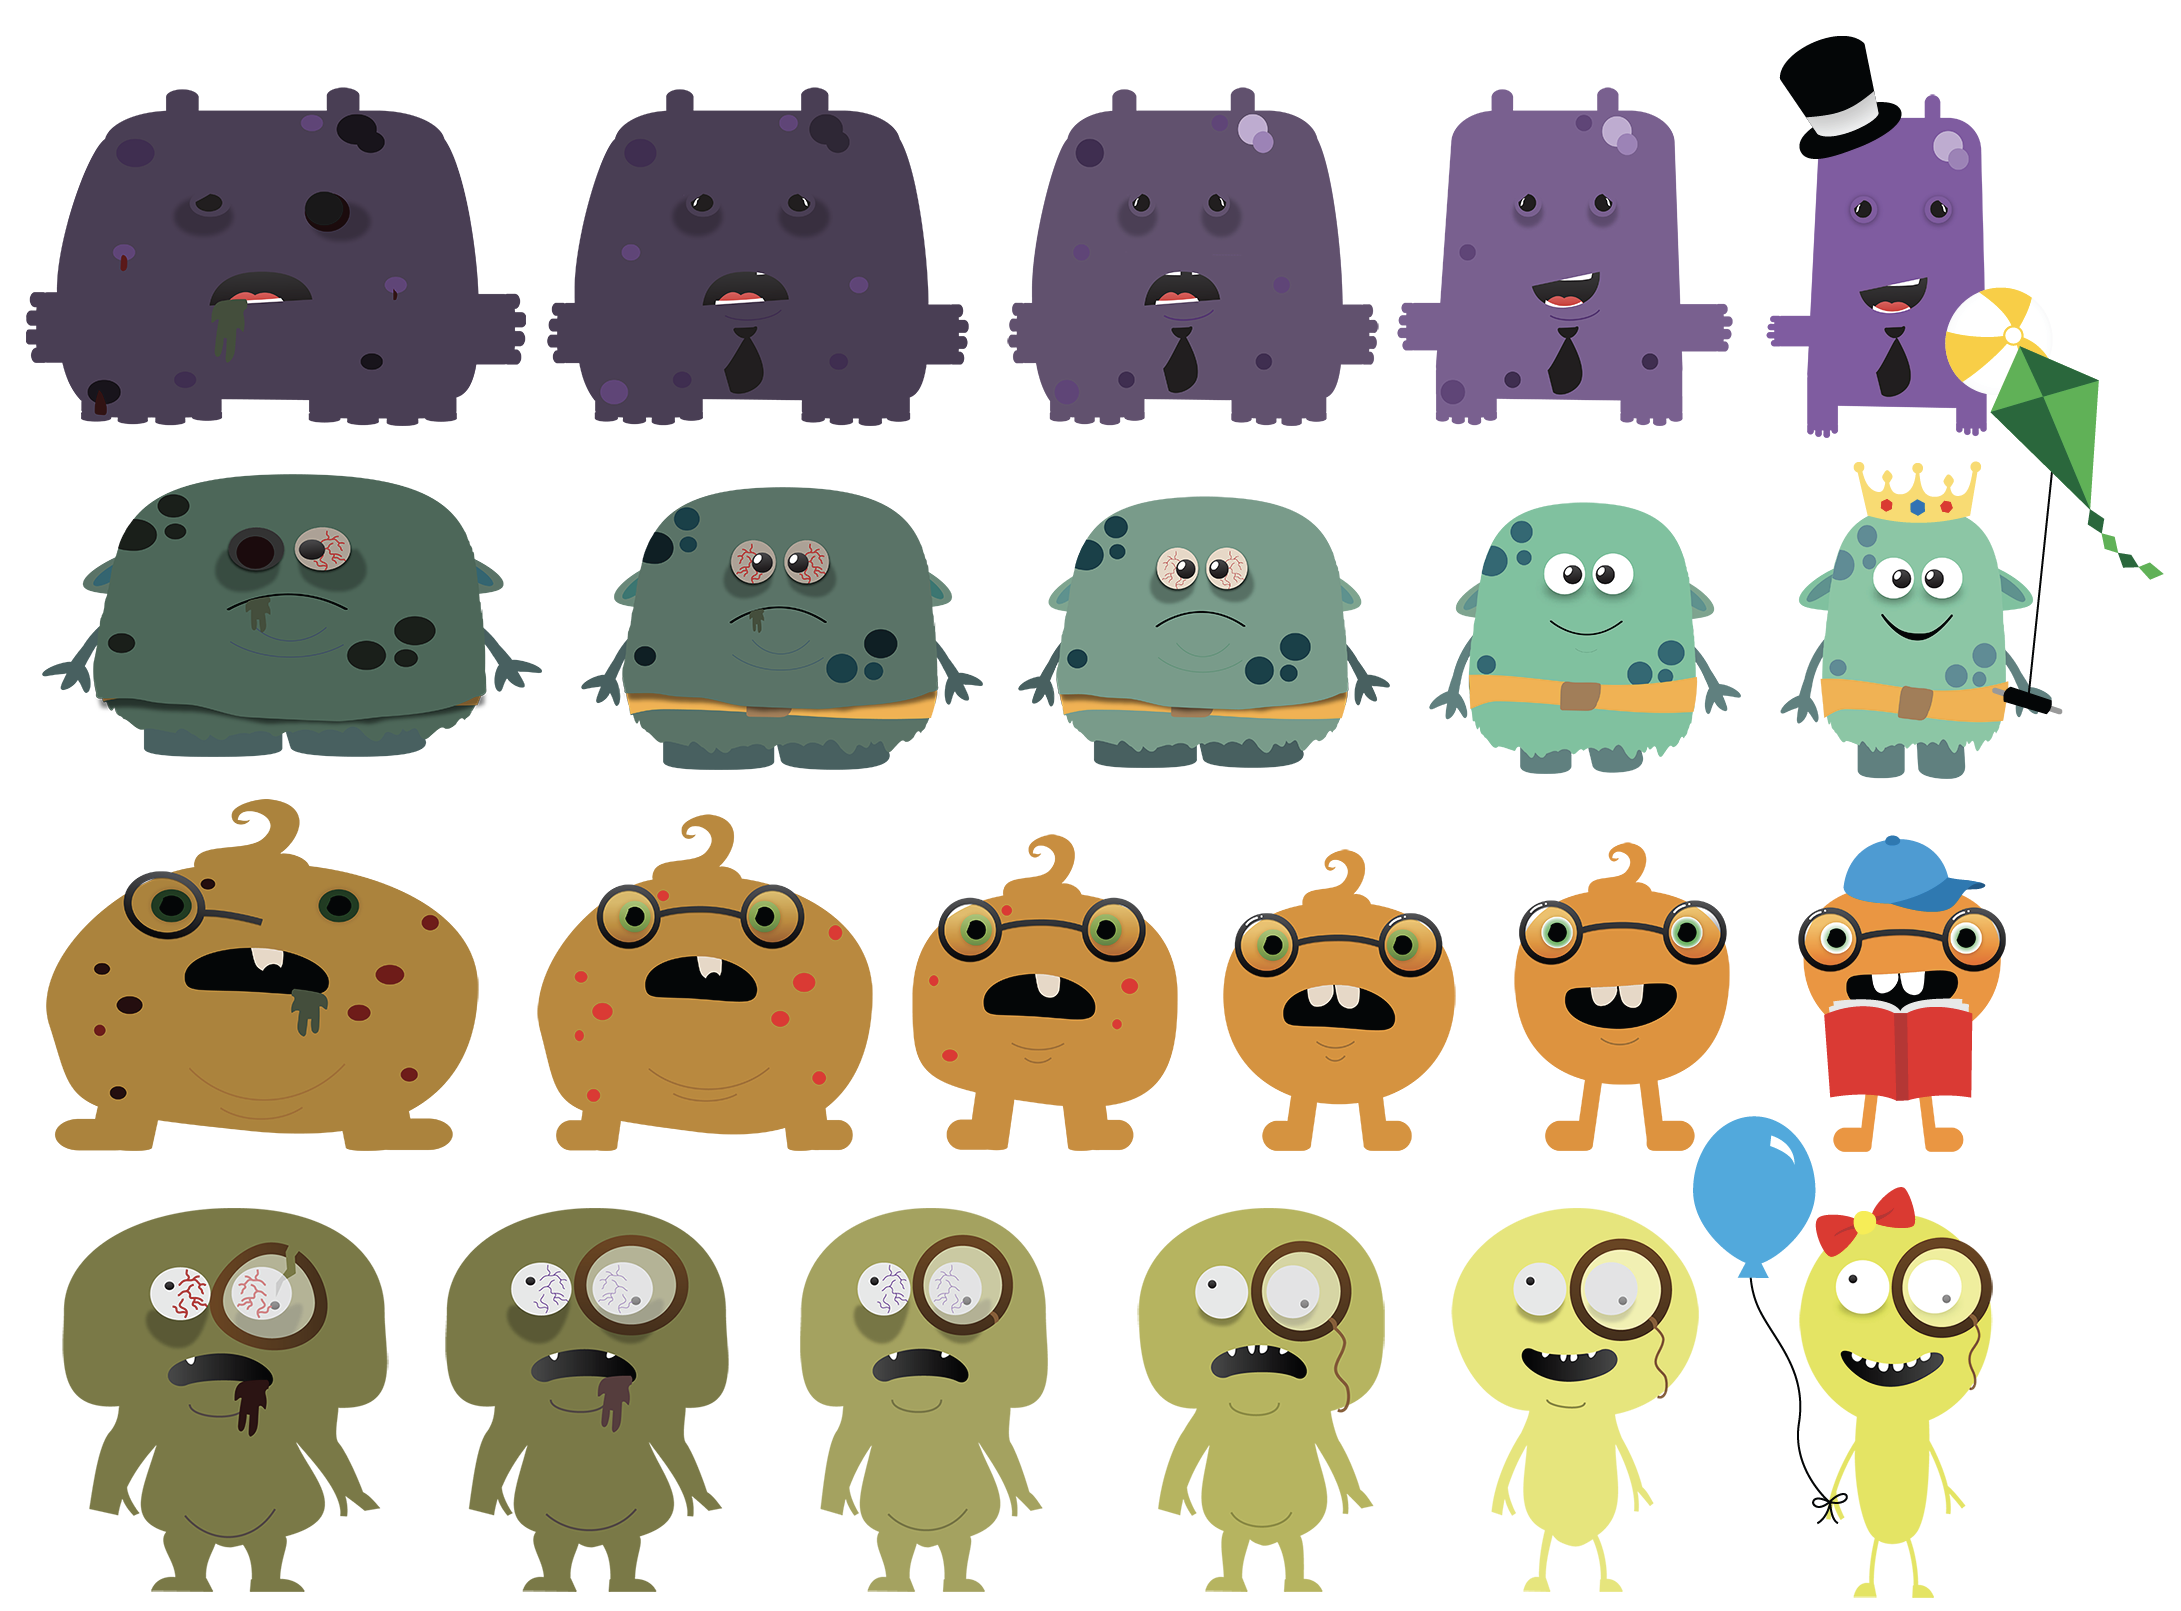
\includegraphics[width=\linewidth]{samples/images/figure-5.png}
\caption{Sample of various monster condition stages and available accessories.}
\label{fig:monster-stages}
\end{wrapfigure}
 
Once the user has viewed the CB and submitted their final meal choice, they will be able to watch their pet monster avatar react to the meal they have chosen to feed them. 
If the monster is fed the best choice meal for their nutritional goal, the user will see their monster avatar's physical state improve in a short animated morph.
If the user feeds their pet monster either the worst meal option, or the second to worst, they will see their pet monster's physical state degrade in the animated morph. 
If the monster is given the second best meal option, their condition neither improves nor worsens. 
%This visual feedback allows the user to see the impact of their choices for their pet monster, as well as motivate them to provide the best options in the future.
This game component also gave users the chance to earn and choose accessories for their pet monster. 
If within the five rounds of ``gameplay'' a user answers four or more questions with the best meal option, the user unlocked the accessories screen, where they were able to choose one of four accessories to award their pet monster. 
Given the five rounds, users could win up to two accessories.







Within the app, in each round, when the four images of meal choices were shown, each was accompanied by a brief description of its contents. 
Users were asked to select the meal option that they believed best fit their monster's nutritional goal. 
The app also prompted users to explain their reasoning for their meal choice.
After submitting their reason, users were told whether or not they selected the best choice and shown the correct answer.
This process of choosing a meal option, providing the reason why, and viewing the result was repeated for each of the five rounds.




\subsection{Development of pre-test and post-test }

The consent form, demographic questionnaire, pre-test assessment, post-test assessment, player-avatar identification questions, and the user experience questions were all created using the online survey platform, Qualtrics.

This is where we will reference Marissa's paper~\cite{burgermaster2017role} a lot -- this was our inspiration (her paper is mentioned in the Observational Learning subsection in the background section). 

+ Elliot's paper~\cite{mitchell2019wish} about carb choices -- we need to reference that too

``Learning outcomes that are seen as relevant to the effectiveness of DGBL are 1) increased interest in the subject matter, 2) improvement in objective performance (e.g., in a test), and 3) transfer, referring to the player's ability to apply acquired knowledge or skills to real-world situations.'' -- referenced from ``Towards a conceptual framework for assessing the effectiveness of digital game-based learning''~\cite{all2015towards}
--- this could be a good rationale for our decision in choosing the recall items (relates to 2) objective performance) and transfer items (relates to 3) transfer). What do you guys think?

We created the pre- and post-task surveys in the online survey platform, Qualtrics.

There were two pre-task surveys, a demographic questionnaire, and a pre-test nutritional assessment.
In the demographic questionnaire, users were asked basic demographic questions and questions about their prior experiences with nutritional knowledge and health related apps. The pre-test nutritional assessment consisted of 12 questions in which users were tasked with identifying which of two meal options better fit a given macronutrient content goal (e.g., which meal photograph is higher in carbohydrates). 
In these 12 questions, the participants did not receive feedback on the accuracy of their responses. 
The 12 questions were made up of 4 questions for each macronutrient (carbs, fat, fiber). 

The post-task consisted of three surveys: the post-test assessment, the player-avatar-identification (PAID) 
The post-test assessment was similar to the pre-task survey in that it was also made up of two parts: 18 questions where the user was asked to identify which of two meal options better fit a given macronutrient content goal, and follow-up questions related to their experience in the study. 
The 18 meal identification questions consisted of 6 questions for each of the three macronutrients, with 4 questions containing meals repeated from the pre-task survey, and 2 questions containing meals that were new to the user. 